% ======================================================
% TÀI LIỆU: Nhóm-PA2-[Tên đồ án] - Use Case Specification
% Môn: CSC13112 - UI/UX Design
% Nội dung: Use Case Specification cho các giải pháp khái niệm
% Tác giả: Nhóm [Tên nhóm]
% Ngày tạo: Tháng 8, 2026
% ======================================================

% --- Định dạng tài liệu ---
% article: tài liệu ngắn (PA, báo cáo), không phân chương (chapter)
% 12pt: cỡ chữ gốc 12pt (đọc dễ chịu trên A4)
% a4paper: khổ giấy A4 (210mm x 297mm)
\documentclass[12pt,a4paper]{article}

% ===================== PACKAGES =====================
% --- Gói hỗ trợ mã hóa và ngôn ngữ ---
\usepackage[utf8]{inputenc}  % Hỗ trợ mã hóa UTF-8 (tiếng Việt, ký hiệu đặc biệt)
\usepackage[T1]{fontenc}     % Bảng mã font T1 - hiển thị dấu tiếng Việt đúng cách
\usepackage[vietnamese]{babel} % Hỗ trợ ngôn ngữ tiếng Việt (phân cách từ, font)

% --- Gói hỗ trợ bố cục và trình bày ---
\usepackage{graphicx}   % Chèn ảnh (\includegraphics)
\usepackage{booktabs}   % Bảng đẹp hơn với \toprule, \midrule, \bottomrule
\usepackage{tabularx}   % Bảng tự động giãn cột theo \textwidth (cột X co giãn)
\usepackage{hyperref}   % Liên kết siêu văn bản (\url, \href), đánh số chương mục
\usepackage{enumitem}   % Tùy chỉnh danh sách (enumerate, itemize) - spacing, bullet style
\usepackage{geometry}   % Đặt lề trang (left, right, top, bottom)
\usepackage{xcolor}     % Hỗ trợ màu sắc (dùng trong hyperref, text color)
\usepackage{titlesec}   % Tùy chỉnh định dạng tiêu đề section
\usepackage{fancyhdr}   % Header/footer tùy chỉnh (trang tiêu, trang cuối)
\usepackage{amssymb}    % Ký hiệu toán học mở rộng
\usepackage[page,toc]{appendix} % Hỗ trợ appendix với environment appendices
\usepackage{pifont}     % Ký hiệu tròn số (\ding{172}=①, \ding{173}=②, \ding{174}=③)
\usepackage{pgfplots}   % Vẽ biểu đồ (charts)
\pgfplotsset{compat=1.18} % Phiên bản pgfplots
\usepackage{tikz}       % Vẽ đồ họa (cho use case diagrams)
\usepackage{tcolorbox}   % Hộp màu (cho use case specifications)

% --- Thư viện TikZ cho use case diagrams ---
\usetikzlibrary{shapes,arrows,positioning,calc}

% --- Thiết lập lề trang ---
% Lề 2.5cm các cạnh: chuẩn cho báo cáo học thuật A4
% left/right: lề trái/phải | top/bottom: lề trên/dưới
\geometry{left=2.5cm, right=2.5cm, top=2.5cm, bottom=2.5cm}

% --- Fix fancyhdr: headheight phải đủ lớn cho header ---
\setlength{\headheight}{15pt}  % Mặc định 12pt quá nhỏ, fancyhdr yêu cầu ≥ 14.93912pt

% --- Cài đặt hyperlink ---
% colorlinks=true: bật màu cho liên kết (thay vì khung viền)
% linkcolor: màu liên kết nội bộ (mục lục, section)
% urlcolor: màu liên kết URL bên ngoài
% citecolor: màu trích dẫn tài liệu tham khảo
\hypersetup{
    colorlinks=true,
    linkcolor=blue,   % Xanh đậm
    urlcolor=blue,   % Đồng bộ với linkcolor
    citecolor=black            % Trích dẫn màu đen (trang trọng)
}

% ===================== HEADER / FOOTER =====================
% fancyhdr: tạo header/footer tùy chỉnh cho tất cả trang
\pagestyle{fancy}         % Kích hoạt chế độ fancy page style
\fancyhf{}                % Xóa tất cả header/footer mặc định
\fancyfoot[C]{\thepage}   % Số trang ở chính giữa footer
% Header
\fancyhead[L]{NHÓM 9} % Trái
\fancyhead[C]{} % Giữa
\fancyhead[R]{23KTPM2} % Phải
\renewcommand{\headrulewidth}{0.4pt}           % Đường kẻ ngang dưới header (0.4pt mảnh)

% ===================== TITLE (TIÊU ĐỀ) =====================
% \title: tiêu đề chính của tài liệu
\title{\textbf{Use Case Specification}}

% --- Định dạng tiêu đề section ---
\titleformat{\section}
{\normalfont\large\bfseries}
{\thesection}{1em}{}

% --- Định dạng tiêu đề phần (trước appendix) ---
\titleformat{\section}{\Large\bfseries}{Part \Roman{section}.}{1em}{}
\titleformat{\subsection}{\normalsize\bfseries}{\thesubsection.}{1em}{}

% --- Cài đặt paragraph ---
\setlength{\parindent}{0pt}
\renewcommand{\contentsname}{Table of contents}

% ===================== USE CASE SPECIFICATION ENVIRONMENTS =====================
% --- Môi trường cho Use Case Specification ---
% Tạo một hộp tcolorbox cho mỗi use case
\newtcolorbox{usecase}[2][]{
    colback=blue!5!white,
    colframe=blue!70!black,
    fonttitle=\bfseries,
    title={#2},
    arc=3pt,
    boxrule=0.8pt,
    left=8pt,
    right=8pt,
    top=6pt,
    bottom=6pt,
    #1  % Các tùy chọn thêm
}

% --- Định dạng cho các mục trong use case ---
\newcommand{\usecasefield}[2]{%
    \textbf{#1:} #2 \par\vspace{2pt}
}

% --- Môi trường cho Main Flow (luồng chính) ---
\newenvironment{mainflow}{
    \par\vspace{4pt}
    \textbf{Main Flow:}
    \begin{enumerate}[leftmargin=*, label=\arabic*., itemsep=2pt]
}{
    \end{enumerate}
}

% --- Môi trường cho Alternative Flows (luồng thay thế) ---
\newenvironment{altflow}{
    \par\vspace{4pt}
    \textbf{Alternative Flows:}
    \begin{itemize}[leftmargin=*, label=\textendash, itemsep=2pt]
}{
    \end{itemize}
}

% ===================== TIKZ STYLES CHO USE CASE DIAGRAMS =====================
% Định dạng cho actor (hình người)
\tikzset{
    actor/.style={
        draw,
        circle,
        minimum size=0.5cm,
        inner sep=0pt,
        fill=gray!20
    },
    usecase/.style={
        draw,
        ellipse,
        minimum width=2cm,
        minimum height=0.8cm,
        text centered,
        fill=blue!10
    },
    system/.style={
        draw,
        rectangle,
        minimum width=6cm,
        minimum height=4cm,
        dashed,
        fill=white
    }
}

% ======================================================
% BẮT ĐẦU NỘI DUNG TÀI LIỆU
% ======================================================
\begin{document}        % Bắt đầu nội dung tài liệu

% ------------ TRANG BÌA -------------
% ------------ TRANG BÌA -------------
\begin{titlepage}
\begin{tikzpicture}[remember picture,overlay,inner sep=0,outer sep=0]
     \draw[blue!70!black,line width=4pt] ([xshift=-1.5cm,yshift=-2cm]current page.north east) coordinate (A)--([xshift=1.5cm,yshift=-2cm]current page.north west) coordinate(B)--([xshift=1.5cm,yshift=2cm]current page.south west) coordinate (C)--([xshift=-1.5cm,yshift=2cm]current page.south east) coordinate(D)--cycle;

     \draw ([yshift=0.5cm,xshift=-0.5cm]A)-- ([yshift=0.5cm,xshift=0.5cm]B)--
     ([yshift=-0.5cm,xshift=0.5cm]B) --([yshift=-0.5cm,xshift=-0.5cm]B)--([yshift=0.5cm,xshift=-0.5cm]C)--([yshift=0.5cm,xshift=0.5cm]C)--([yshift=-0.5cm,xshift=0.5cm]C)-- ([yshift=-0.5cm,xshift=-0.5cm]D)--([yshift=0.5cm,xshift=-0.5cm]D)--([yshift=0.5cm,xshift=0.5cm]D)--([yshift=-0.3cm,xshift=0.5cm]A)--([yshift=-0.3cm,xshift=-0.5cm]A)--([yshift=0.5cm,xshift=-0.5cm]A);


     \draw ([yshift=-0.3cm,xshift=0.3cm]A)-- ([yshift=-0.3cm,xshift=-0.3cm]B)--
     ([yshift=0.3cm,xshift=-0.3cm]B) --([yshift=0.3cm,xshift=0.3cm]B)--([yshift=-0.3cm,xshift=0.3cm]C)--([yshift=-0.3cm,xshift=-0.3cm]C)--([yshift=0.3cm,xshift=-0.3cm]C)-- ([yshift=0.3cm,xshift=0.3cm]D)--([yshift=0.3cm,xshift=0.3cm]D)--([yshift=-0.3cm,xshift=-0.3cm]D)--([yshift=0.3cm,xshift=-0.3cm]A)--([yshift=0.3cm,xshift=0.3cm]A)--([yshift=-0.3cm,xshift=-0.3cm]A);

\end{tikzpicture}
\vspace*{1cm}
\begin{center}
    \makebox[\textwidth][c]{\large\bfseries ĐẠI HỌC QUỐC GIA THÀNH PHỐ HỒ CHÍ MINH}\\[4pt]
    \makebox[\textwidth][c]{\large\bfseries TRƯỜNG ĐẠI HỌC KHOA HỌC TỰ NHIÊN - VNUHCM}\\[4pt]
    \makebox[\textwidth][c]{\large\bfseries KHOA CÔNG NGHỆ THÔNG TIN}\\[1cm]
    

    
\includegraphics[scale=0.15]{Logo-Dai-hoc-Khoa-hoc-Tu-nhien.png}\\[0.8cm]
    % Môn học
    {\large\bfseries THIẾT KẾ GIAO DIỆN}

    \vspace{6pt}

    {\large Lớp: \textbf{23KTPM2}}
    
    \vspace{10pt}
    
    % Tiêu đề đồ án (một dòng, màu, to, căn giữa)
    \makebox[\textwidth][c]{\large\bfseries \color{black!70!black}USE CASE SPECIFICATION - PA2}
    
    \vspace{1.5cm}

    % Giáo viên box
    \begin{tcolorbox}[colback=blue!5!white, colframe=blue!50!black, width=0.9\textwidth, boxrule=0.8pt, arc=3pt, left=8pt, right=8pt]
        \textbf{Thầy: Lê Khánh Duy}\\
        \textbf{Thầy: Nguyễn Huy Khánh}\\
        \textbf{Thầy: Phạm Nguyễn Sơn Tùng}
    \end{tcolorbox}
    \vspace{1cm}

    % Sinh viên box
    \begin{tcolorbox}[colback=gray!10!white, colframe=gray!60!black, width=0.9\textwidth, boxrule=0.8pt, arc=3pt, left=8pt, right=8pt]
        \textbf{Sinh viên thực hiện:} \\
        Huỳnh Lê Khôi -- MSSV: 23127068 \\ 
        Bùi Đức Đạt -- MSSV: 23127337 \\
        Phan Thị Hương Xuân -- MSSV: 23127147 \\
        Nguyễn Tuấn Minh -- MSSV: 22127271 \\
        Nguyễn Hồng Phúc -- MSSV: 22127333
        
    \end{tcolorbox}

    \vfill
    {\large\textbf{HO CHI MINH CITY, 2026}}
\end{center}
\end{titlepage}


\tableofcontents        % Tự động tạo mục lục từ các \section, \subsection
\newpage                % Ngắt trang - mục lục ở trang riêng

% ======================================================
% PHẦN I: GIỚI THIỆU
% ======================================================
\section{Giới thiệu}

% Mô tả mục đích của tài liệu Use Case Specification
% Giải thích cách sử dụng tài liệu này
% Liệt kê các giải pháp khái niệm được đề cập (dựa trên PA2 Requirement 3)

% ======================================================
% PHẦN II: VẤN ĐỀ 1 — TRÌ HOẠN KHI XEM TRỰC TIẾP
% ======================================================
\section{Vấn đề 1: Trì hoãn khi xem trực tiếp}

\subsection{Concept A: Phân đoạn nội dung bằng AI}

% Mô tả ngắn gọn về giải pháp AI phân đoạn nội dung

\subsubsection{Sơ đồ Use Case}

\begin{figure}[htbp]
    \centering
    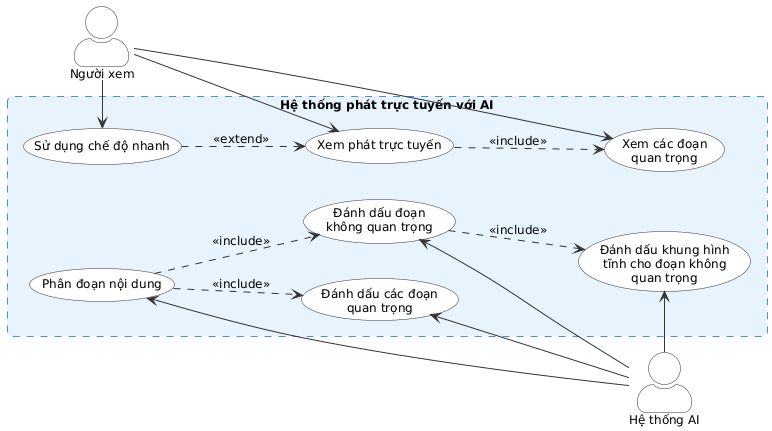
\includegraphics[width=0.8\textwidth]{usecase-diagrams/uc-ai-segmentation.png}
    \caption{Sơ đồ Use Case cho Concept A: Phân đoạn nội dung bằng AI}
    \label{fig:uc-ai-segmentation}
\end{figure}

\subsubsection{Đặc tả Use Case}

\begin{usecase}{UC1: Xem phát trực tuyến}
    \usecasefield{Actor}{Người xem}
    \usecasefield{Mục tiêu}{Xem nội dung phát trực tuyến}
    \usecasefield{Điều kiện tiên quyết}{Luồng trực tuyến đang hoạt động, Người xem có kết nối internet}
    \begin{mainflow}
        \item Người xem mở ứng dụng phát trực tuyến
        \item Người xem chọn luồng trực tuyến để xem
        \item Hệ thống tải và hiển thị luồng trực tuyến
    \end{mainflow}
    \begin{altflow}
        \item Nếu xảy ra trì hoãn, hệ thống có thể gợi ý bật chế độ nhanh
    \end{altflow}
    \usecasefield{Điều kiện kết quả}{Người xem đang xem phát trực tuyến}
\end{usecase}

\begin{usecase}{UC2: Xem các đoạn quan trọng}
    \usecasefield{Actor}{Người xem}
    \usecasefield{Mục tiêu}{Di chuyển nhanh đến các phần quan trọng của luồng trực tuyến}
    \usecasefield{Điều kiện tiên quyết}{AI đã phân đoạn nội dung, Các đoạn quan trọng đã được đánh dấu}
    \begin{mainflow}
        \item Người xem thấy các đoạn đã đánh dấu trên timeline
        \item Người xem nhấp vào đoạn đã đánh dấu
        \item Hệ thống nhảy đến đoạn đó
    \end{mainflow}
    \begin{altflow}
        \item Nếu chưa có đoạn nào được đánh dấu, người xem xem luồng bình thường
    \end{altflow}
    \usecasefield{Điều kiện kết quả}{Người xem đang xem đoạn quan trọng}
\end{usecase}

\begin{usecase}{UC3: Sử dụng chế độ nhanh}
    \usecasefield{Actor}{Người xem}
    \usecasefield{Mục tiêu}{Xem nội dung không quan trọng ở định dạng rút gọn}
    \usecasefield{Điều kiện tiên quyết}{AI đã xử lý nội dung, Chế độ nhanh khả dụng}
    \begin{mainflow}
        \item Người xem bật chế độ nhanh
        \item Hệ thống hiển thị hình ảnh tĩnh với văn bản và âm thanh
        \item Văn bản phát liên tục để mô phỏng cập nhật theo thời gian thực
    \end{mainflow}
    \begin{altflow}
        \item Nếu là người xem đầu tiên, chế độ nhanh có thể chưa khả dụng
    \end{altflow}
    \usecasefield{Điều kiện kết quả}{Người xem nhận được bản cập nhật thông tin rút gọn}
\end{usecase}

\begin{usecase}{UC4: Phân đoạn nội dung}
    \usecasefield{Actor}{Hệ thống AI}
    \usecasefield{Mục tiêu}{Tự động phân tích và chia luồng trực tuyến thành các đoạn quan trọng và không quan trọng}
    \usecasefield{Điều kiện tiên quyết}{Luồng trực tuyến đang hoạt động, AI đã được huấn luyện}
    \begin{mainflow}
        \item Hệ thống AI phân tích lời bình luận và hình ảnh trong video
        \item Hệ thống xác định ranh giới giữa các đoạn quan trọng và không quan trọng
        \item Hệ thống lưu kết quả phân đoạn
    \end{mainflow}
    \begin{altflow}
        \item Nếu dữ liệu quá lớn, hệ thống phân đoạn theo batch
    \end{altflow}
    \usecasefield{Điều kiện kết quả}{Luồng trực tuyến đã được phân đoạn thành công}
\end{usecase}

\begin{usecase}{UC5: Đánh dấu các đoạn quan trọng}
    \usecasefield{Actor}{Hệ thống AI}
    \usecasefield{Mục tiêu}{Gắn nhãn đánh dấu cho các đoạn nội dung quan trọng}
    \usecasefield{Điều kiện tiên quyết}{Nội dung đã được phân đoạn (UC4)}
    \begin{mainflow}
        \item Hệ thống xác định đoạn nào là quan trọng dựa trên phân tích
        \item Hệ thống gắn nhãn ``quan trọng'' cho các đoạn đó
        \item Hệ thống cập nhật timeline hiển thị
    \end{mainflow}
    \begin{altflow}
        \item Nếu không có đoạn quan trọng nào, hệ thống không đánh dấu gì
    \end{altflow}
    \usecasefield{Điều kiện kết quả}{Các đoạn quan trọng đã được đánh dấu trên timeline}
\end{usecase}

\begin{usecase}{UC7: Đánh dấu đoạn không quan trọng}
    \usecasefield{Actor}{Hệ thống AI}
    \usecasefield{Mục tiêu}{Xác định và đánh dấu các đoạn nội dung không quan trọng}
    \usecasefield{Điều kiện tiên quyết}{Nội dung đã được phân đoạn (UC4)}
    \begin{mainflow}
        \item Hệ thống xác định các đoạn không quan trọng dựa trên phân tích
        \item Hệ thống gắn nhãn ``không quan trọng'' cho các đoạn đó
        \item Hệ thống chuẩn bị dữ liệu cho chế độ nhanh
    \end{mainflow}
    \begin{altflow}
        \item Nếu tất cả đều quan trọng, hệ thống không đánh dấu gì
    \end{altflow}
    \usecasefield{Điều kiện kết quả}{Các đoạn không quan trọng đã được đánh dấu}
\end{usecase}

\begin{usecase}{UC8: Đánh dấu khung hình tĩnh cho đoạn không quan trọng}
    \usecasefield{Actor}{Hệ thống AI}
    \usecasefield{Mục tiêu}{Chọn và gắn khung hình tĩnh đại diện cho mỗi đoạn không quan trọng}
    \usecasefield{Điều kiện tiên quyết}{Các đoạn không quan trọng đã được đánh dấu (UC7)}
    \begin{mainflow}
        \item Hệ thống quét qua từng đoạn không quan trọng
        \item Hệ thống chọn khung hình có chất lượng tốt nhất (độ rõ, ánh sáng)
        \item Hệ thống lưu khung hình tĩnh làm ảnh đại diện cho đoạn đó
    \end{mainflow}
    \begin{altflow}
        \item Nếu không tìm được khung hình phù hợp, hệ thống dùng khung hình mặc định
    \end{altflow}
    \usecasefield{Điều kiện kết quả}{Mỗi đoạn không quan trọng có kèm khung hình tĩnh}
\end{usecase}

\subsection{Concept B: Gọi video P2P giữa các người dùng}

% Mô tả ngắn gọn về giải pháp P2P gọi video

\subsubsection{Sơ đồ Use Case}

\begin{figure}[htbp]
    \centering
    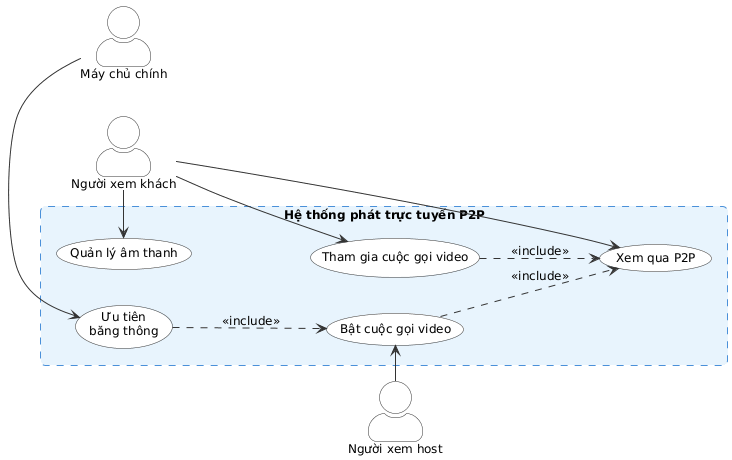
\includegraphics[width=0.8\textwidth]{usecase-diagrams/uc-p2p-calling.png}
    \caption{Sơ đồ Use Case cho Concept B: Gọi video P2P}
    \label{fig:uc-p2p-calling}
\end{figure}

\subsubsection{Đặc tả Use Case}

\begin{usecase}{UC1: Bật cuộc gọi video}
    \usecasefield{Actor}{Người xem host}
    \usecasefield{Mục tiêu}{Chia sẻ luồng trực tuyến qua gọi video P2P}
    \usecasefield{Điều kiện tiên quyết}{Đang xem luồng trực tuyến, Tính năng P2P khả dụng}
    \begin{mainflow}
        \item Hệ thống hiển thị thông báo mời bật cuộc gọi video
        \item Người xem host đồng ý bật tính năng gọi video
        \item Hệ thống thiết lập kết nối P2P và bắt đầu chia sẻ luồng
    \end{mainflow}
    \begin{altflow}
        \item Nếu người xem host từ chối, hệ thống tiếp tục phát trực tuyến bình thường
    \end{altflow}
    \usecasefield{Điều kiện kết quả}{Cuộc gọi video P2P đang hoạt động, luồng được chia sẻ}
\end{usecase}

\begin{usecase}{UC2: Tham gia cuộc gọi video}
    \usecasefield{Actor}{Người xem khách}
    \usecasefield{Mục tiêu}{Tham gia xem luồng trực tuyến qua kết nối P2P}
    \usecasefield{Điều kiện tiên quyết}{Có người xem host đang chia sẻ luồng, Mạng P2P khả dụng}
    \begin{mainflow}
        \item Hệ thống hiển thị tùy chọn ``Tham gia P2P''
        \item Người xem khách chọn tham gia
        \item Hệ thống kết nối với luồng của host
    \end{mainflow}
    \begin{altflow}
        \item Nếu không có host nào khả dụng, hệ thống chuyển về xem từ server
    \end{altflow}
    \usecasefield{Điều kiện kết quả}{Người xem khách đang xem qua P2P}
\end{usecase}

\begin{usecase}{UC3: Xem qua P2P}
    \usecasefield{Actor}{Người xem khách}
    \usecasefield{Mục tiêu}{Nhận và xem luồng video từ host}
    \usecasefield{Điều kiện tiên quyết}{Đã tham gia cuộc gọi P2P (UC2)}
    \begin{mainflow}
        \item Hệ thống nhận luồng video từ host
        \item Hệ thống giải mã và hiển thị video
        \item Người xem khách xem nội dung
    \end{mainflow}
    \begin{altflow}
        \item Nếu mất kết nối P2P, hệ thống tự động chuyển về server
    \end{altflow}
    \usecasefield{Điều kiện kết quả}{Người xem khách đang xem video}
\end{usecase}

\begin{usecase}{UC4: Ưu tiên băng thông}
    \usecasefield{Actor}{Máy chủ chính}
    \usecasefield{Mục tiêu}{Cấp băng thông ưu tiên cho các kết nối P2P}
    \usecasefield{Điều kiện tiên quyết}{Có kết nối P2P đang hoạt động}
    \begin{mainflow}
        \item Hệ thống phát hiện kết nối P2P
        \item Hệ thống cấp băng thông ưu tiên cho kết nối đó
        \item Hệ thống theo dõi và điều chỉnh băng thông theo thời gian thực
    \end{mainflow}
    \begin{altflow}
        \item Nếu băng thông không đủ, hệ thống giảm chất lượng video
    \end{altflow}
    \usecasefield{Điều kiện kết quả}{Băng thông P2P được ưu tiên}
\end{usecase}

\begin{usecase}{UC5: Quản lý âm thanh}
    \usecasefield{Actor}{Người xem khách}
    \usecasefield{Mục tiêu}{Tắt tiếng hoặc điều chỉnh âm thanh từ các người dùng khác}
    \usecasefield{Điều kiện tiên quyết}{Đang trong cuộc gọi video P2P}
    \begin{mainflow}
        \item Người xem khách mở bảng điều khiển âm thanh
        \item Người xem khách chọn tắt tiếng các người dùng khác
        \item Hệ thống tắt âm thanh từ các nguồn đó
    \end{mainflow}
    \begin{altflow}
        \item Người xem khách có thể điều chỉnh âm lượng thay vì tắt hoàn toàn
    \end{altflow}
    \usecasefield{Điều kiện kết quả}{Chỉ còn nghe âm thanh từ luồng chính}
\end{usecase}

% ======================================================
% PHẦN III: VẤN ĐỀ 2 — QUÁ TẢI THÔNG TIN
% ======================================================
\section{Vấn đề 2: Quá tải thông tin cho người dùng mới}

\subsection{Concept A: Giảm banner và carousel}

% Mô tả ngắn gọn về giải pháp giảm banner/carousel

\subsubsection{Sơ đồ Use Case}

\begin{figure}[htbp]
    \centering
    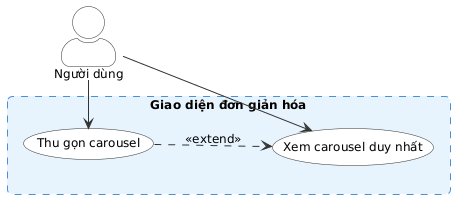
\includegraphics[width=0.8\textwidth]{usecase-diagrams/uc-reduce-banners.png}
    \caption{Sơ đồ Use Case cho Concept A: Giảm banner/carousel}
    \label{fig:uc-reduce-banners}
\end{figure}

\subsubsection{Đặc tả Use Case}

\begin{usecase}{UC1: Xem carousel duy nhất}
    \usecasefield{Actor}{Người dùng}
    \usecasefield{Mục tiêu}{Duyệt nội dung nổi bật thông qua carousel đơn giản}
    \usecasefield{Điều kiện tiên quyết}{Người dùng đã mở ứng dụng}
    \begin{mainflow}
        \item Hệ thống hiển thị carousel duy nhất ở thanh bên
        \item Carousel tự động chuyển slide với nội dung nổi bật
        \item Người dùng tương tác để xem chi tiết hoặc xem slide tiếp
    \end{mainflow}
    \begin{altflow}
        \item Nếu không có nội dung nổi bật, carousel hiển thị thông báo ``Không có nội dung mới''
    \end{altflow}
    \usecasefield{Điều kiện kết quả}{Người dùng đã xem nội dung từ carousel}
\end{usecase}

\begin{usecase}{UC2: Thu gọn carousel}
    \usecasefield{Actor}{Người dùng}
    \usecasefield{Mục tiêu}{Ẩn carousel để mở rộng không gian hiển thị nội dung chính}
    \usecasefield{Điều kiện tiên quyết}{Carousel đang hiển thị}
    \begin{mainflow}
        \item Người dùng nhấp nút ``Thu gọn'' trên carousel
        \item Hệ thống ẩn carousel với hiệu ứng trượt
        \item Không gian màn hình mở rộng cho nội dung chính
    \end{mainflow}
    \begin{altflow}
        \item Người dùng có thể mở lại carousel bằng nút ``Mở rộng''
    \end{altflow}
    \usecasefield{Điều kiện kết quả}{Carousel đã được ẩn, nội dung chính chiếm toàn màn hình}
\end{usecase}

\subsection{Concept B: Chế độ chỉnh sửa với kéo thả}

% Mô tả ngắn gọn về giải pháp chỉnh sửa giao diện

\subsubsection{Sơ đồ Use Case}

\begin{figure}[htbp]
    \centering
    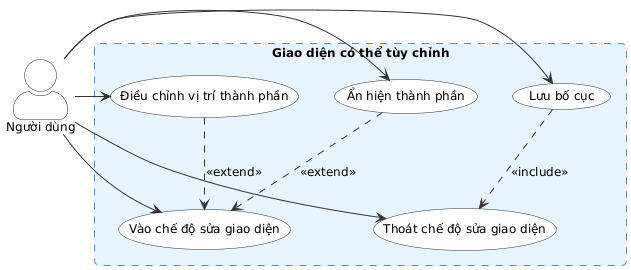
\includegraphics[width=0.8\textwidth]{usecase-diagrams/uc-edit-mode.png}
    \caption{Sơ đồ Use Case cho Concept B: Chế độ chỉnh sửa với kéo thả}
    \label{fig:uc-edit-mode}
\end{figure}

\subsubsection{Đặc tả Use Case}

\begin{usecase}{UC1: Vào chế độ sửa giao diện}
    \usecasefield{Actor}{Người dùng}
    \usecasefield{Mục tiêu}{Chuyển sang chế độ cho phép tùy chỉnh bố cục giao diện}
    \usecasefield{Điều kiện tiên quyết}{Người dùng đang ở màn hình chính}
    \begin{mainflow}
        \item Người dùng nhấp nút ``Chỉnh sửa'' ở góc màn hình
        \item Hệ thống hiển thị overlay chỉnh sửa với các điểm kéo thả
        \item Giao diện chuyển sang trạng thái có thể tùy chỉnh
    \end{mainflow}
    \begin{altflow}
        \item Nếu không có thay đổi, hệ thống không lưu khi thoát
    \end{altflow}
    \usecasefield{Điều kiện kết quả}{Giao diện đang ở chế độ chỉnh sửa}
\end{usecase}

\begin{usecase}{UC2: Thoát chế độ sửa giao diện}
    \usecasefield{Actor}{Người dùng}
    \usecasefield{Mục tiêu}{Rời khỏi chế độ chỉnh sửa và lưu các thay đổi}
    \usecasefield{Điều kiện tiên quyết}{Đang ở chế độ chỉnh sửa (UC1)}
    \begin{mainflow}
        \item Người dùng nhấp nút ``Xong'' hoặc ``Lưu''
        \item Hệ thống lưu lại bố cục mới
        \item Giao diện trở về trạng thái bình thường với bố cục mới
    \end{mainflow}
    \begin{altflow}
        \item Người dùng có thể chọn ``Hủy'' để không lưu thay đổi
    \end{altflow}
    \usecasefield{Điều kiện kết quả}{Bố cục giao diện đã được lưu}
\end{usecase}

\begin{usecase}{UC3: Lưu bố cục}
    \usecasefield{Actor}{Người dùng}
    \usecasefield{Mục tiêu}{Lưu lại vị trí và trạng thái hiển thị của các thành phần}
    \usecasefield{Điều kiện tiên quyết}{Đang ở chế độ chỉnh sửa, Đã thực hiện thay đổi}
    \begin{mainflow}
        \item Người dùng nhấp nút ``Lưu bố cục''
        \item Hệ thống ghi lại vị trí của từng thành phần
        \item Hệ thống lưu cấu hình vào tài khoản người dùng
    \end{mainflow}
    \begin{altflow}
        \item Nếu chưa có thay đổi, nút lưu bị vô hiệu hóa
    \end{altflow}
    \usecasefield{Điều kiện kết quả}{Bố cục đã được lưu thành công}
\end{usecase}

\begin{usecase}{UC4: Ẩn hiện thành phần}
    \usecasefield{Actor}{Người dùng}
    \usecasefield{Mục tiêu}{Ẩn hoặc hiển thị các thành phần trên giao diện}
    \usecasefield{Điều kiện tiên quyết}{Đang ở chế độ chỉnh sửa (UC1)}
    \begin{mainflow}
        \item Người dùng nhấp vào biểu tượng mắt trên thành phần
        \item Hệ thống ẩn thành phần (hoặc hiển thị lại nếu đang ẩn)
        \item Giao diện tự động điều chỉnh bố cục
    \end{mainflow}
    \begin{altflow}
        \item Người dùng có thể ẩn nhiều thành phần cùng lúc
    \end{altflow}
    \usecasefield{Điều kiện kết quả}{Trạng thái hiển thị của thành phần đã thay đổi}
\end{usecase}

\begin{usecase}{UC5: Điều chỉnh vị trí thành phần}
    \usecasefield{Actor}{Người dùng}
    \usecasefield{Mục tiêu}{Di chuyển các thành phần đến vị trí mới trên giao diện}
    \usecasefield{Điều kiện tiên quyết}{Đang ở chế độ chỉnh sửa (UC1)}
    \begin{mainflow}
        \item Người dùng giữ và kéo thành phần đến vị trí mới
        \item Hệ thống hiển thị vùng thả hợp lệ
        \item Người dùng thả thành phần, hệ thống cập nhật bố cục
    \end{mainflow}
    \begin{altflow}
        \item Nếu vị trí mới trùng với thành phần khác, hệ thống hoán đổi vị trí
    \end{altflow}
    \usecasefield{Điều kiện kết quả}{Thành phần đã di chuyển đến vị trí mới}
\end{usecase}

% ======================================================
%          BIBLIOGRAPHY (Chưa có citation - bật lại khi thêm \cite{})
% ======================================================
% \bibliographystyle{plain}
% \bibliography{references}

% % ======================================================
% %          PHỤ LỤC
% % ======================================================
% \newpage
% \appendix
% \appendixpage
% \addappheadtotoc

\end{document}
